
\documentclass[12pt]{article}
\setlength\parindent{0pt}
\usepackage{fullpage}
\usepackage{amsmath}
\usepackage[margin=1in]{geometry}
\usepackage{graphicx}
\setlength{\parskip}{4mm}
\def\LL{\left\langle}   % left angle bracket
\def\RR{\right\rangle}  % right angle bracket
\def\LP{\left(}         % left parenthesis
\def\RP{\right)}        % right parenthesis
\def\LB{\left\{}        % left curly bracket
\def\RB{\right\}}       % right curly bracket
\def\PAR#1#2{ {{\partial #1}\over{\partial #2}} }
\def\PARTWO#1#2{ {{\partial^2 #1}\over{\partial #2}^2} }
\def\PARTWOMIX#1#2#3{ {{\partial^2 #1}\over{\partial #2 \partial #3}} }
\newcommand{\BE}{\begin{displaymath}}
\newcommand{\EE}{\end{displaymath}}
\newcommand{\BNE}{\begin{equation}}
\newcommand{\ENE}{\end{equation}}
\newcommand{\BEA}{\begin{eqnarray}}
\newcommand{\EEA}{\nonumber\end{eqnarray}}
\newcommand{\EL}{\nonumber\\}
\newcommand{\la}[1]{\label{#1}}
\newcommand{\ie}{{\em i.e.\ }}
\newcommand{\eg}{{\em e.\,g.\ }}
\newcommand{\cf}{cf.\ }
\newcommand{\etc}{etc.\ }
\newcommand{\Tr}{{\rm tr}}
\newcommand{\etal}{{\it et al.}}
\newcommand{\OL}[1]{\overline{#1}\ } % overline
\newcommand{\OLL}[1]{\overline{\overline{#1}}\ } % double overline
\newcommand{\OON}{\frac{1}{N}} % "one over N"
\newcommand{\OOX}[1]{\frac{1}{#1}} % "one over X"

\pagenumbering{gobble}

\begin{document}
\Large
\centerline{\sc{Recitation Exercises -- Work and Potential Energy}}
\normalsize
\centerline{\sc{Week 9, Day 2}}
%
%
%{A rock climber of mass 70 kg is climbing a cliff face when she slips and falls. She is two meters above her last anchor, so she will undergo free fall for 4 meters before the rope begins to arrest her fall. If the stiffness in her rope is 1400 N/m, then:}
%  \begin{enumerate}
%    \item{How far will she fall in total?}
%\vspace{2in}
%
%    \item{What is the maximum force that her rope will exert on her as it arrests her fall?}
%\vspace{1.5in}
%
%    \item When would it be desirable for a rock climber to use a rope with a large spring constant? What about a smaller spring constant? You'll need to think about 
%          the engineering reasons for climbers to use ropes at all: the goal is to minimize the forces involved in arresting a climber's fall.
%   \end{enumerate}
%
%\newpage
%%
%% \item{A laptop battery says it has a capacity of 51 ``watt-hours''.}
%%   \begin{enumerate}
%%     \item{What are the dimensions of this odd unit ``watt-hour'', and what does it measure? What is 51 watt-hours in more familiar units?}
%%
%%\vspace{2.5in}
%%
%%     \item{If this battery were used to power an electric motor, how high could it lift the battery? Assume the battery has a mass of 300 grams.}
%%\vspace{2.5in}
%%   \end{enumerate}
%%
%%\newpage

\begin{center}
	\small \it If you didn't get to this problem during the first recitation this week, do it today.
\end{center}

 An object rests at bottom of an incline that is elevated at an angle $\theta$ above the horizontal. Suppose that there is no friction at first. A person slides this object up the incline; it travels a distance $D$ up the incline before it slides back down.

\begin{enumerate}

\item What forces act on the object? Determine whether each one does positive work, negative work, or zero work on the way up and on the way down.

\vspace{2in}

\item	Suppose at first there is no friction. What initial velocity does the person have to slide it with for it to travel a distance $D$ before it begins to slide back down? 

\vspace{2.5in}

\item	When it reaches the base of the incline again, how will its velocity compare to the initial velocity that it had on the way up? {\it (You should be able to answer this without doing any mathematics.)}

\vspace{2in}

\newpage

\item	Now, suppose that there is friction -- a coefficient of friction $\mu_k$ between the ramp and the object. 
What initial velocity would the person have to slide it with {\it now} for it to travel a distance $D$ before it comes back down?

\vspace{3in}


\item How fast will it be moving {\it now} when it reaches the bottom of the ramp? 

\vspace{3.7in}

\item If an object travels through some path but comes back to where it starts, like in this case, a force that always does zero work is a {\it conservative force}. A force that does do work when an object travels along a closed path is a {\it nonconservative force}.

Three forces appear in this problem: a normal force, gravity, and friction. Is each of these a conservative force? Why or why not?

\end{enumerate}
\newpage

\begin{center}
	\it This exercise is arguably the most important one to understand fully for the energy section on Exam 3. If your group has questions here, make sure you ask them!
\end{center}

 
 A child is swinging on a tire swing hanging from a tree. The swing has a length $L$, and the
 	tire plus the child have a mass $m$.
 	
 	The child's older sibling pulls the swing back to an angle $\theta$ and releases it from position A.
 	
 	However, a strong wind is blowing from left to right, exerting a constant horizontal force $F_w$ on the swing to the right. This means that it will swing to a larger angle $\phi$ on the right (at position~C) than it started on the left.




 	\begin{center}
 		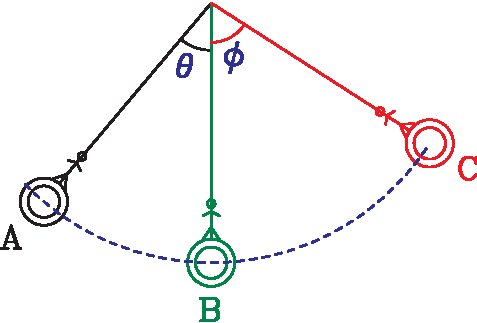
\includegraphics[width=0.6\textwidth]{swing-crop.pdf}
 	\end{center}

 
   \begin{enumerate}
 	\item Write an equation for the work-energy theorem as the swing moves from A to B. Label in words what each term represents, using language as ``kinetic energy at point A'', ``potential energy at point B'', or ``work done by wind in moving from A to B''.
 	
 	\vspace{3in}
 	
 	\newpage
 	\item Find the speed of the swing at position B in terms of $F_w$, $m$, $L$, $\theta$, and $g$.
 	
 	\vspace{2in}
 
 	\item Write down an equation that you could solve for the angle $\phi$ in terms of $F_w$, $m$, $L$, $\theta$, and $g$. (You do not need to actually solve it.) As before, label each term that appears in your expression for the work-energy theorem.
 	
 	
 	\vspace{4in}
 	
 	\item When the tire swings back to the left, will it stop at position $A$, will it move further to the left, or will it not reach position $A$ at all? In deciding this, think about the work done by each force as the tire swings from A to C and then back to A. Call your coach or TA over to discuss with your group.
 \end{enumerate}
 

\newpage


\begin{minipage}{0.4\textwidth}
	
Mt. Wrightson is the tallest peak in the Santa Rita Mountains in southern Arizona, around 40 km north of the border with Mexico.

\bigskip
	
The usual hike up the mountain starts at around 1650 meters altitude and ends at the summit at 2850 meters.
\bigskip



Human muscles convert chemical potential energy in the food we eat into both mechanical work and heat. Depending on the type of motion, the efficiency of this motion can be as high as 25\%. Since walking is quite efficient, suppose that a hiker traveling up this mountain has an efficiency of 20\%. 

\bigskip



\end{minipage}
\hspace{0.05\textwidth}
\begin{minipage}{0.5\textwidth}
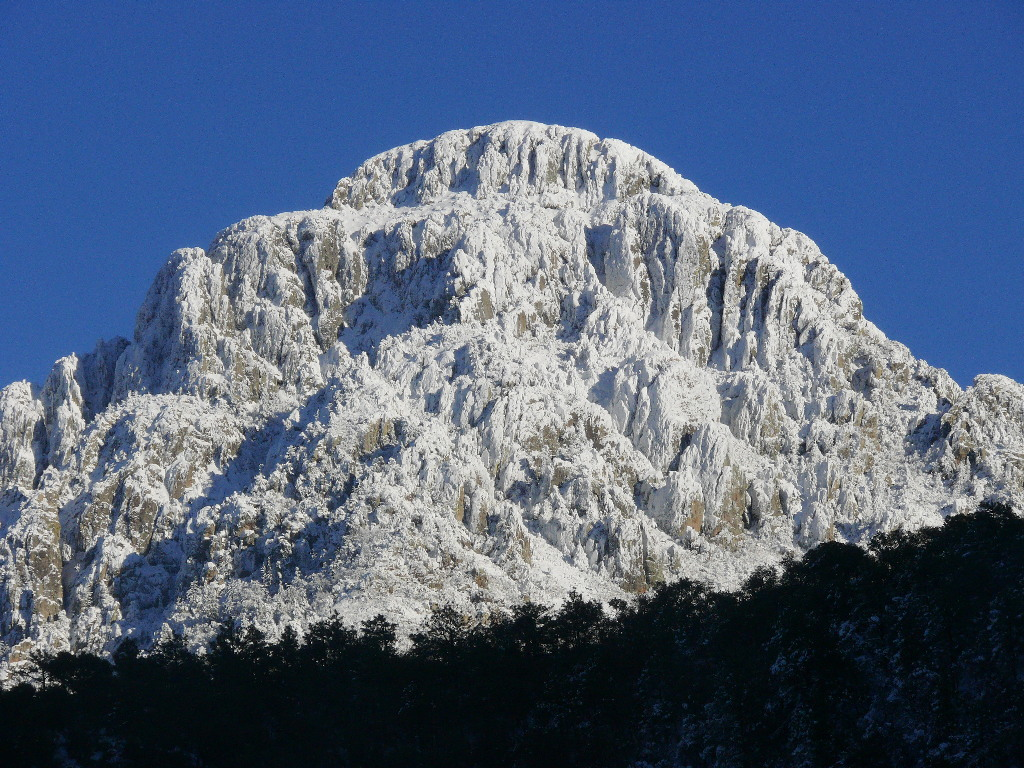
\includegraphics[width=\textwidth]{wrightson1024.jpg}
\end{minipage}


This means that to produce one joule of mechanical work, the hiker's metabolism must extract five joules of chemical potential energy from food; the other four joules of chemical potential energy are converted into heat (which the hiker must get rid to avoid overheating).


\begin{enumerate}
	\item Suppose a hiker climbs Mt. Wrightson carrying a backpack with food, water, and camping equipment. How much mechanical work must their muscles do on them for them to make it to the summit? {\it (You will need to estimate the mass of the hiker and their gear.)}
	\newpage 
	\item How many joules of chemical potential energy must they metabolize to make this climb?
	\vspace{1in}
	\item We often measure food energy in ``kilocalories'' (or ``Calories'', with a capital letter, confusing everyone); one kcal is equal to 4180 J. How many kcal must our hiker extract from their food to make the climb?
	\vspace{1in}
	\item An apple is about 100 kcal; a Clif Bar is about 250 kcal; a big peanut butter and jelly sandwich might be 400 kcal. Is this around the amount of food you'd expect would be needed to fuel this climb?
		\vspace{1in}
		
	\item How much heat will the hiker's metabolism produce in the process?
	\vspace{1in}
	
	\item On a warm day, we cool ourselves during exercise mostly by evaporating sweat. The evaporation of 1 milliliter of water (with a mass of 1 gram) removes around 2500 J of heat. How much water must our hiker drink in order to make it up Mt. Wrightson?
	
\end{enumerate}


 \end{document}
